\subsection{Decision Logic}

% [ERIC/KARTHIK - 1 pg]

% Decision logic, tabular spec and evolution, APT synth and proof \\

% might want to cite Alessandro's recent APT/ATJ/ATC papers?

A critical component of the RTA is the plan selector, which dispatches on candidate flight paths according to a formally verified decision logic. The Collins RTA SWC assessment forwards the plan selector two plans, generated by the LEC and a baseline-avoidance function (BAF) respectively. After running the logic, the plan selector sends its decision (LEC/BAF plan) to the aircraft plan switcher.

% update prose of table summary

Given some combination of the two plans, an assessment is made over five general variables: plan validity, plan safety, time of closest point of approach (tCPA) $> 179$ seconds (establishing a horizon beyond which a plan is meaningless), predicted miss distance comparison between the plans, and plan recency relative to the current time. If a plan is not valid, we deem it unfit for publication. However, if a plan is valid, and we've yet to receive a second plan (we are out of the 3-second recency period), we go ahead and publish said plan. If neither plan is safe, we publish the one with the larger predicted miss distance. So as to highlight the capabilities of the LEC, tie-breaking, in the case of two ideal plans (see row 11 of \ref{fig:selection-logic}), is performed by defaulting to the LEC plan. In the case that we've received two safe plans, we consider each plans' calculated tCPA and if it is projected to be past the 180-second horizon, we disregard said plan and publish the other one. If both plans' tCPAs are beyond the 180-second horizon, we publish the plan with the greater predicted miss distance. See \ref{fig:selection-logic} for the full table.

This table is then encoded into the ACL2 (A Computational Logic for Applicative Common Lisp) theorem prover \cite{acl2} using the $\verb+def-table+$ machinery described in \cite{dasc2020}. Proofs of completeness (an output is always produced) and unambiguity (a unique output is always produced) are automatically generated, ensuring the logic has no immediate inconsistencies.

\begin{figure*}
	\centering
	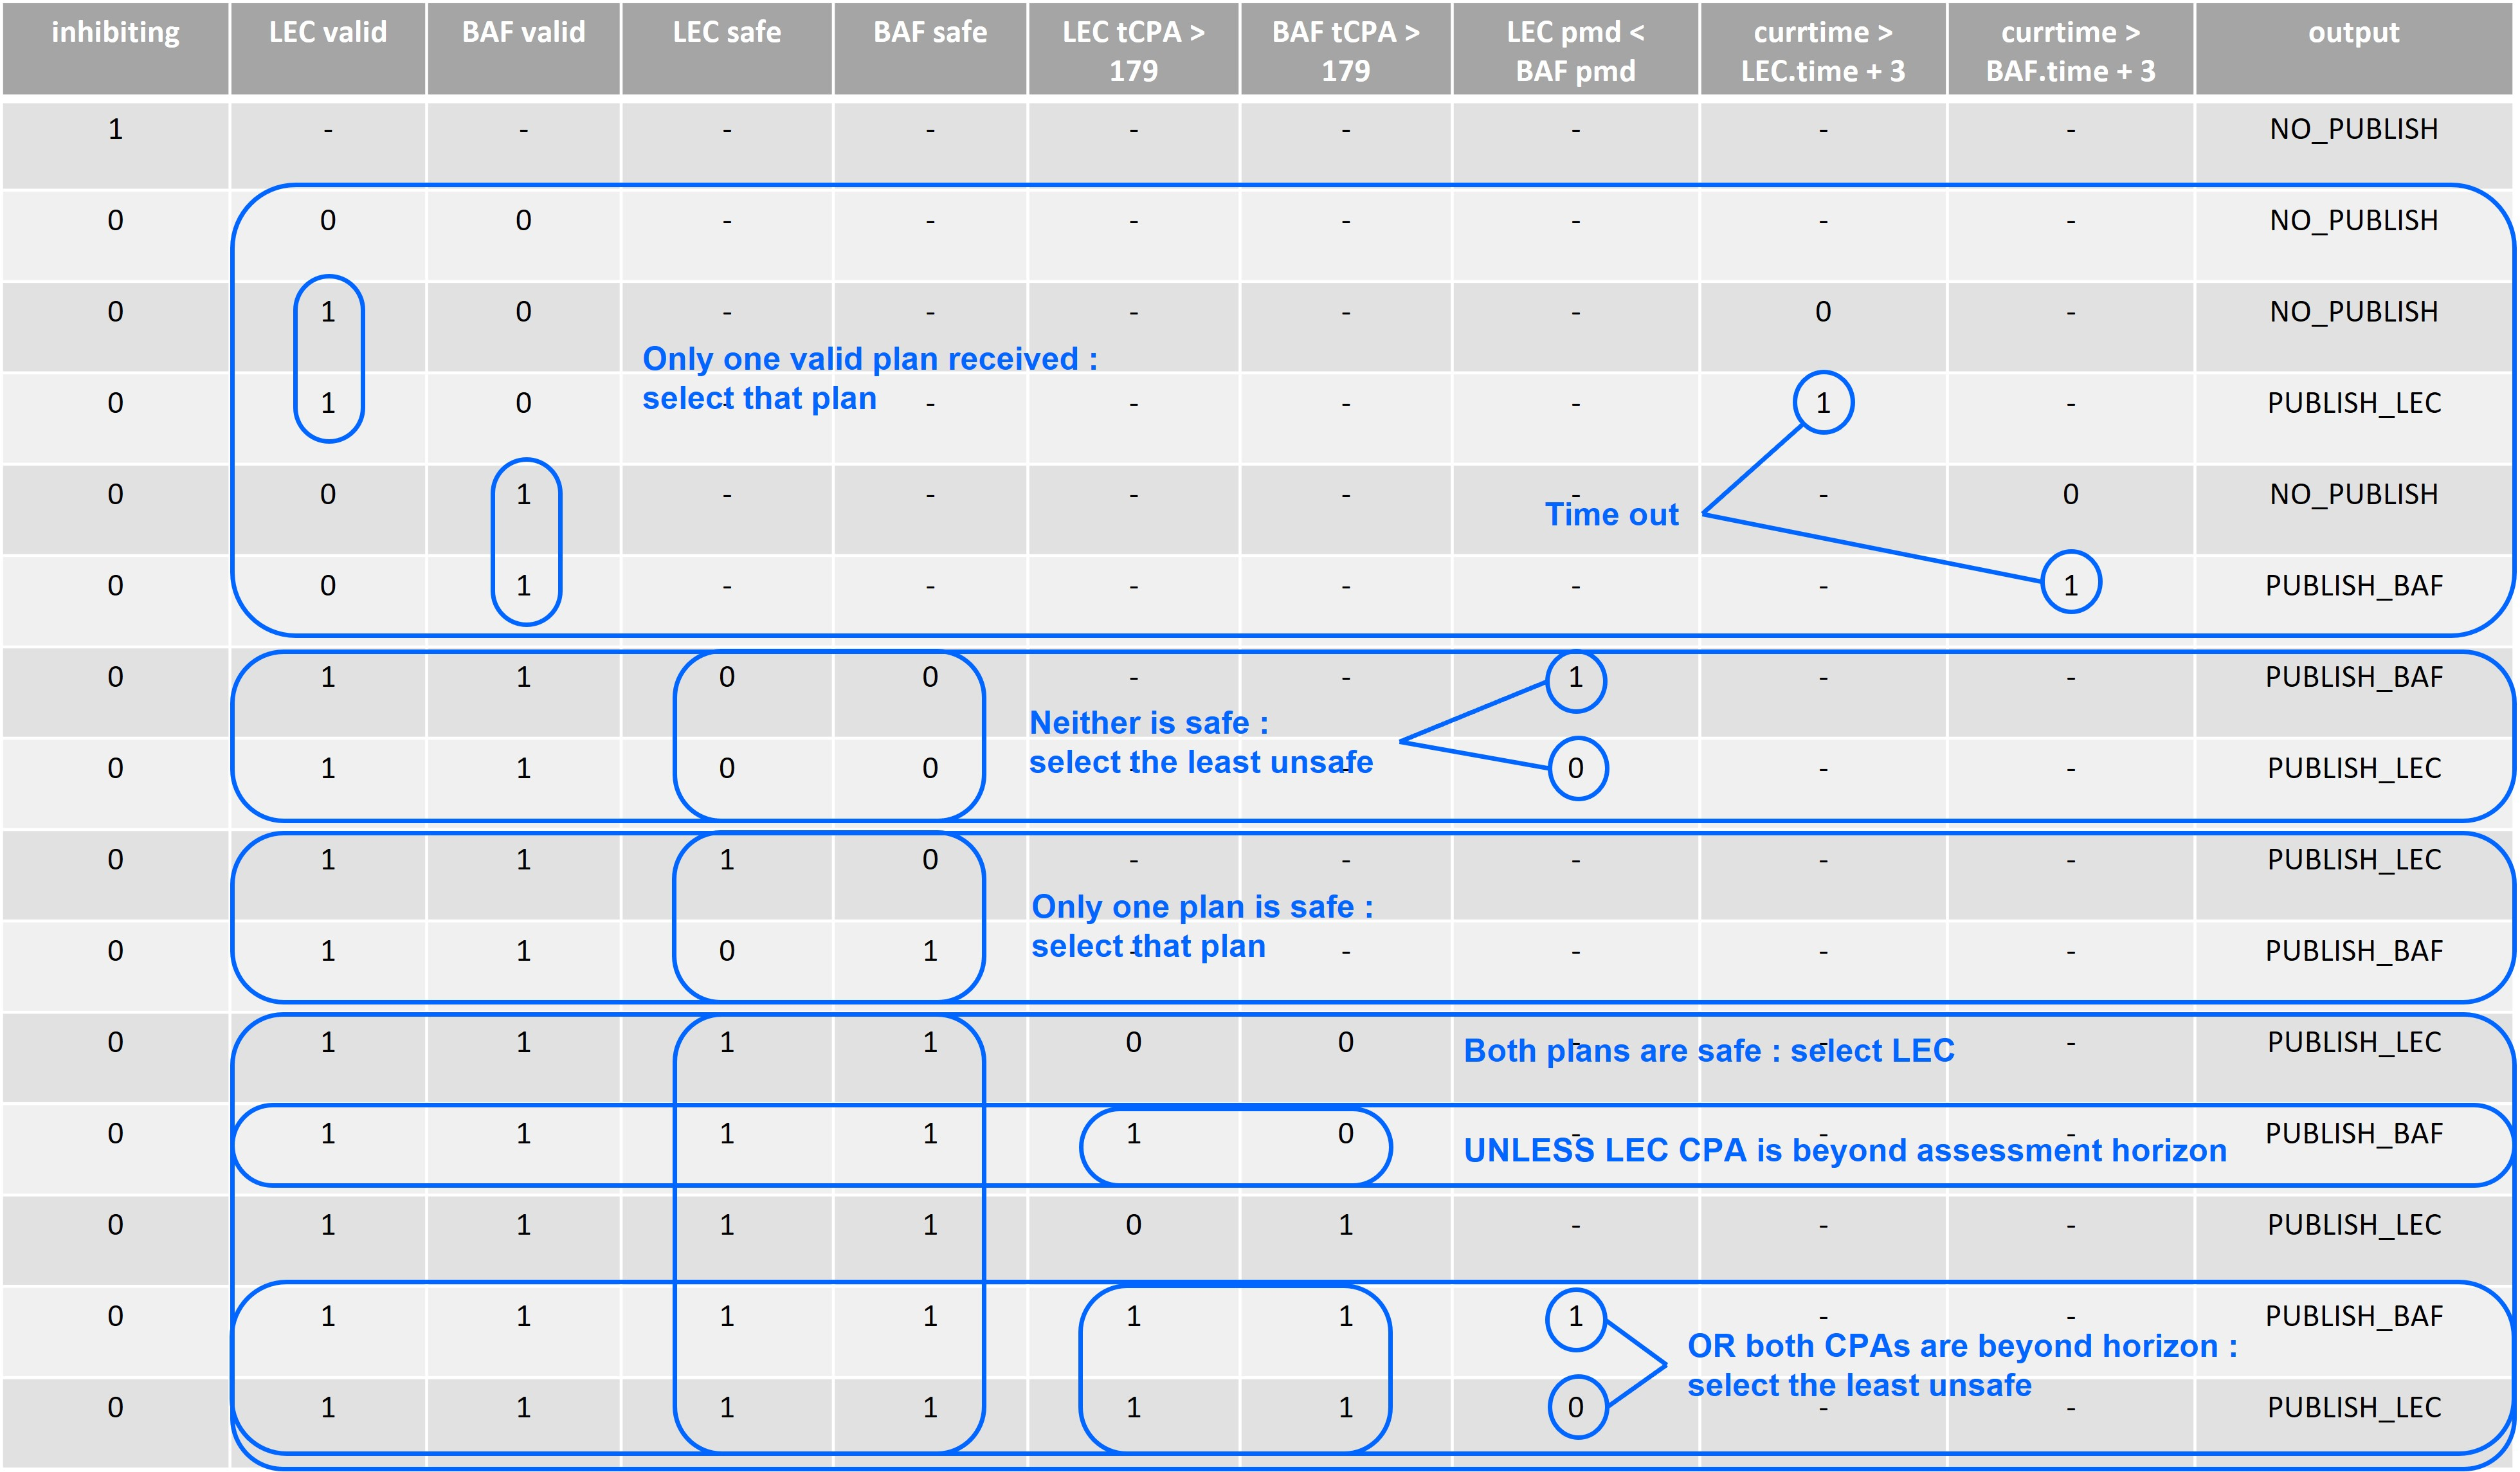
\includegraphics[width=\textwidth]{figures/selection-logic.jpg}
	\caption{Selection Logic behavior specification table}
	\label{fig:selection-logic}
\end{figure*}

% check if we have any other highlights during synthesis

The table serves as the initial formal specification from which we synthesize an executable Java program in two key steps:
\begin{enumerate}
\item \underline{APT optimization/rewriting}: We use Kestrel's APT (Automated Program Transformations) \cite{apt} toolkit, itself built upon ACL2, to transform a direct simulation of the table (using $\verb+apply-table+$ from our table library) into an optimized function. This is accomplished through APT utilities such as $\verb+simplify+$ and logical rewrite rules. Each of the APT transformation steps is equipped with a proof-of-equivalence (of the pre-transformation and post-transformation code). This logic is then transformed into a form admissible for the ATJ code generator using additional APT utilities.
\item \underline{ATJ Java code generation}: We use Kestrel's ATJ (ACL2-to-Java) Java code generator, itself built upon ACL2, to generate Java code for integration with the Collins RTA. Extending previous work, ATJ now generates idiomatic Java code, contrasting the presentation in \cite{dasc2020}, where the code relied heavily on Java classes representing ACL2 values. This optimization eliminates any overhead caused by non-native values and improves usability/readability.
\end{enumerate}

% look through svn logs during Iron Bird simulations and update accordingly

This methodology lends itself to a high degree of flexibility and automates the programming workflow upon any change to the specification. Simulations had necessitated additional conditions and constraints on plan publishing, which simply amounted to changing the $\verb+def-table+$ encoding in ACL2, with all the correctness proofs, synthesis/optimization steps, and Java code generation following immediately.


Directions for further development of this methodology include:
\begin{itemize}
\item \underline{outfitting ATJ with proofs}: As remarked in \cite{dasc2020}, this might involve either formalizing the semantics of Java or using Kestrel's Axe toolkit to lift Java bytecode into logic.
\item \underline{code generation for other languages (C, Python, Rust)}: Recent work at Kestrel was able to achieve the same synthesis presented above using the ATC C code generator in place of ATJ, with the additional benefit of having proofs-of-correctness for the code generation.
\item \underline{formal synthesis of RTA-logic interface}: At the time of publication, the integration of the plan selection logic with the Collins RTA requires a handwritten wrapper, which could potentially also be synthesized with proofs.
\end{itemize}